\documentclass[xcolor=svgnames]{beamer}\usepackage[]{graphicx}\usepackage[]{color}
%% maxwidth is the original width if it is less than linewidth
%% otherwise use linewidth (to make sure the graphics do not exceed the margin)
\makeatletter
\def\maxwidth{ %
  \ifdim\Gin@nat@width>\linewidth
    \linewidth
  \else
    \Gin@nat@width
  \fi
}
\makeatother

\definecolor{fgcolor}{rgb}{0.345, 0.345, 0.345}
\newcommand{\hlnum}[1]{\textcolor[rgb]{0.686,0.059,0.569}{#1}}%
\newcommand{\hlstr}[1]{\textcolor[rgb]{0.192,0.494,0.8}{#1}}%
\newcommand{\hlcom}[1]{\textcolor[rgb]{0.678,0.584,0.686}{\textit{#1}}}%
\newcommand{\hlopt}[1]{\textcolor[rgb]{0,0,0}{#1}}%
\newcommand{\hlstd}[1]{\textcolor[rgb]{0.345,0.345,0.345}{#1}}%
\newcommand{\hlkwa}[1]{\textcolor[rgb]{0.161,0.373,0.58}{\textbf{#1}}}%
\newcommand{\hlkwb}[1]{\textcolor[rgb]{0.69,0.353,0.396}{#1}}%
\newcommand{\hlkwc}[1]{\textcolor[rgb]{0.333,0.667,0.333}{#1}}%
\newcommand{\hlkwd}[1]{\textcolor[rgb]{0.737,0.353,0.396}{\textbf{#1}}}%

\usepackage{framed}
\makeatletter
\newenvironment{kframe}{%
 \def\at@end@of@kframe{}%
 \ifinner\ifhmode%
  \def\at@end@of@kframe{\end{minipage}}%
  \begin{minipage}{\columnwidth}%
 \fi\fi%
 \def\FrameCommand##1{\hskip\@totalleftmargin \hskip-\fboxsep
 \colorbox{shadecolor}{##1}\hskip-\fboxsep
     % There is no \\@totalrightmargin, so:
     \hskip-\linewidth \hskip-\@totalleftmargin \hskip\columnwidth}%
 \MakeFramed {\advance\hsize-\width
   \@totalleftmargin\z@ \linewidth\hsize
   \@setminipage}}%
 {\par\unskip\endMakeFramed%
 \at@end@of@kframe}
\makeatother

\definecolor{shadecolor}{rgb}{.97, .97, .97}
\definecolor{messagecolor}{rgb}{0, 0, 0}
\definecolor{warningcolor}{rgb}{1, 0, 1}
\definecolor{errorcolor}{rgb}{1, 0, 0}
\newenvironment{knitrout}{}{} % an empty environment to be redefined in TeX

\usepackage{alltt}
\usetheme{Boadilla}
\usecolortheme[named=SeaGreen]{structure}
\usepackage{graphicx}
\usepackage{breqn}
\usepackage{xcolor}
\usepackage{booktabs}
\usepackage{verbatim}
\usepackage{tikz}
\usepackage{lmodern}
\usetikzlibrary{shadows,arrows,positioning}
\definecolor{links}{HTML}{2A1B81}
\hypersetup{colorlinks,linkcolor=links,urlcolor=links}
\usepackage{pgfpages}

\newcommand{\Bigtxt}[1]{\textbf{\textit{#1}}}
\IfFileExists{upquote.sty}{\usepackage{upquote}}{}
\begin{document}

\title[R Resources]{List of R Resources}

\author[M. Beck, T. O'Brien]{Marcus W. Beck\inst{1} \and Todd D. O'Brien\inst{2}}

\date{}

\institute[]{\inst{1} ORISE, USEPA NHEERL Gulf Ecology Division\\ Email: \href{mailto:beck.marcus@epa.gov}{beck.marcus@epa.gov} \and \inst{2} NOAA/NMFS COPEPOD Project\\ Email: \href{todd.obrien@noaa.gov}{todd.obrien@noaa.gov}}

% knitr setup


% load SWMPr from local


%%%%%%
\begin{frame}
\vspace{0.3in}
\centerline{
\begin{tikzpicture}
  \node[drop shadow={shadow xshift=0ex,shadow yshift=0ex},fill=white,draw] at (0,0) {
\includegraphics[width=0.9\textwidth]{bg_main.jpg}};
\end{tikzpicture}}
\titlepage
\end{frame}

%%%%%%
\begin{frame}[t]{R Resources}
All of the course material is available on the website: \href{http://copepod.org/nerrs-swmp-workshop/}{http://copepod.org/nerrs-swmp-workshop/}\\~\\

\begin{itemize}
\item Pre-workshop toolkit
\item Training modules - presentations, scripts, datasets
\item SWMP cookbook and supplementary materials \\~\\
\end{itemize}

The SWMPr package will continue to be developed - eventually submitted to CRAN \\
~\\
Check the SWMPr \href{https://github.com/fawda123/SWMPr}{GitHub page} for ongoing development \\~\\
Feedback, suggestions, bugs, harsh criticism - email Marcus at beck.marcus@epa.gov
\end{frame}

%%%%%%
\begin{frame}{R Resources}
The \href{http://cran.r-project.org/doc/contrib/Short-refcard.pdf}{R reference card}:\\~\\
\centerline{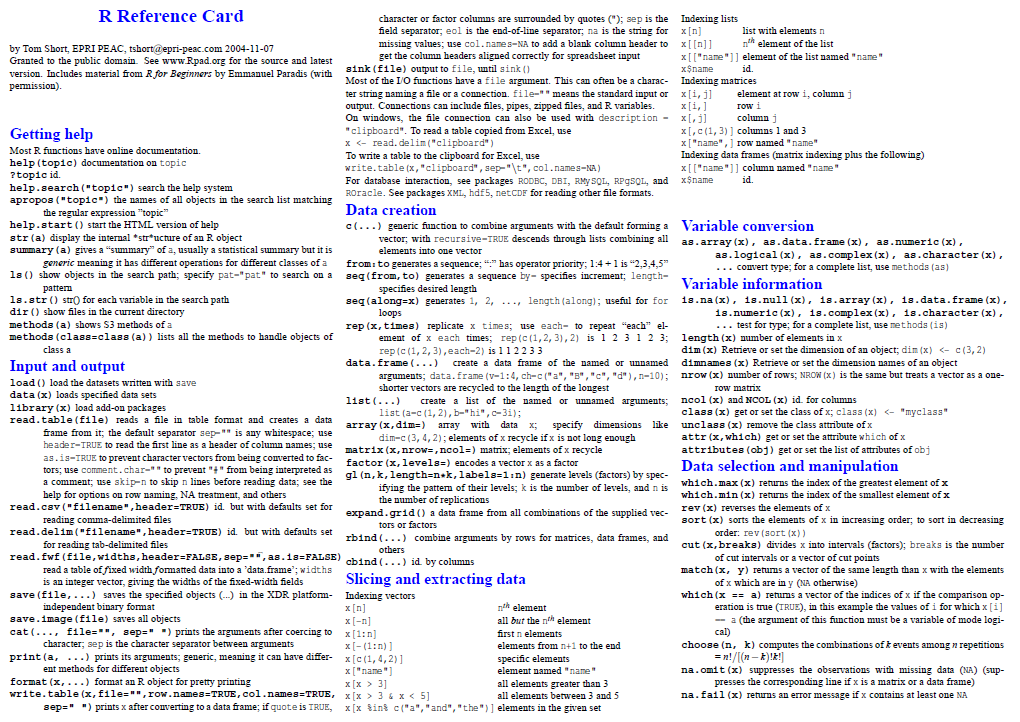
\includegraphics[width = 0.8\textwidth]{r_ref_card.png}}
\end{frame}

%%%%%%
\begin{frame}[t]{R Resources}
The \href{http://cran.r-project.org/doc/contrib/Torfs+Brauer-Short-R-Intro.pdf}{Short R introduction}:\\~\\
\vfill
\centerline{
\includegraphics[width = 0.6\textwidth]{r_tutorial.png}}
\vfill
\end{frame}

%%%%%%
\begin{frame}[t]{R Resources}
The \href{http://cran.r-project.org/doc/contrib/Torfs+Brauer-Short-R-Intro.pdf}{Short R introduction}:\\~\\
\begin{columns}[T]
\begin{column}{0.5\textwidth}
\centerline{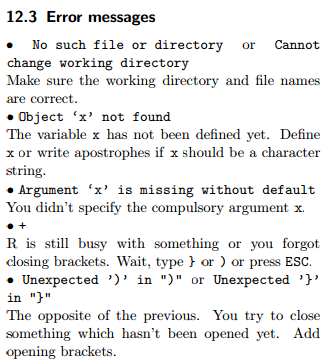
\includegraphics[width = 0.8\textwidth]{err1.png}}
\end{column}
\begin{column}{0.5\textwidth}
\centerline{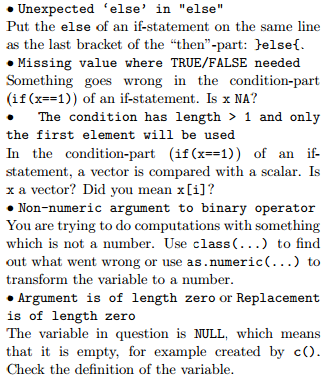
\includegraphics[width = 0.8\textwidth]{err2.png}}
\end{column}
\end{columns}
\end{frame}

%%%%%%
\begin{frame}[t]{R Resources}
\begin{columns}
\begin{column}{0.5\textwidth}
\begin{itemize}
\item Getting data into R 
\item Accessing variables and subsets
\item Simple functions
\item Loops
\item Graphing
\item Introduction to the Lattice package
\item Common mistakes
\end{itemize}
\end{column}
\begin{column}{0.5\textwidth}
\centerline{
\includegraphics[width = 0.8\textwidth]{book3.jpeg}}
\end{column}
\end{columns}
\end{frame}

%%%%%%
\begin{frame}[t]{R Resources}
The \href{http://cran.r-project.org/doc/manuals/R-intro.html}{CRAN R tutorial} (detailed):\\~\\
\vfill
\centerline{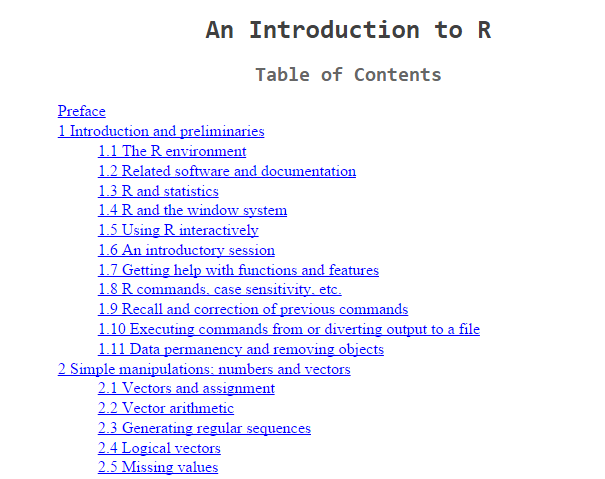
\includegraphics[width = 0.6\textwidth]{cran_intro.png}}
\vfill
\end{frame}

%%%%%%
\begin{frame}[t]{R Resources}
My suggested help workflow: \\~\\
\begin{enumerate}
\item Check the help file for a function - usually the syntax is incorrect. \\~\\
\item Check online - A Google search of the problem will usually return an answer.  Best to use the actual error message as a search term. \\~\\
\item Ask a real person that knows about R - I try to be as responsive as possible to emails. \\~\\
\item Post online, e.g., \href{http://stackoverflow.com/}{Stack Overflow} or \href{https://stat.ethz.ch/mailman/listinfo/r-help}{R-help}, usually only after all other options are exhausted.  Make sure you follow posting guidelines.\\~\\
\item Do not give up!
\end{enumerate}
\end{frame}

%%%%%%
\begin{frame}[t]{R Resources}
Final comments about learning R:\\~\\
\begin{itemize}
\item R is becoming the de facto statistical analysis program - soon your mom will be using R \\~\\
\item R will fundamentally change how you work with data \\~\\
\item You determine the flow of the analysis, not the other way around \\~\\
\item Time spent banging your head on the wall is time spent learning \\~\\
\item Initial time investments will have huge returns - you will become more efficient \\~\\
\item Do not give up!
\end{itemize}
\end{frame}

\end{document}
